\documentclass[a4paper, 10pt]{article}

%% Language and font encodings
\usepackage[english]{babel}
\usepackage[utf8]{inputenc}
\usepackage[T1]{fontenc}

%% Sets page size and margins
\usepackage[a4paper,top=2.5cm,bottom=2.3cm,left=2.5cm,right=1.9cm]{geometry}


%% Useful packages
\usepackage{amsmath}
\usepackage{siunitx}
\usepackage{booktabs}
\usepackage{graphicx}
\usepackage[colorinlistoftodos]{todonotes}
\usepackage[colorlinks=true, allcolors=blue]{hyperref}
\usepackage{subcaption}
\usepackage{multirow}
\usepackage{arydshln}  % dashed lines
\usepackage{changepage}
\usepackage{blindtext} % lorem ipsum

\renewcommand{\arraystretch}{1.25} % for tables

\title{Artificial Neural Networks reports}
\author{Mauro Paradela del Río - r0696150}
\date{}

\begin{document}
\maketitle
\newpage
\section{Lab 1}
  \subsection{Algorithm comparison}
  \begin{table}[h!]
    \begin{tabular}{@{}lrrrr@{}}
      \toprule
      \multicolumn{5}{c}{\textbf{gd}} \\
      N  &   $R_t$  &  $MSE_t$ &  Epch  & T(s)\\
      \midrule
      10       &   0.06     &  0.49       &  771     & 2.64   \\
      20       &   0.31     &  0.37       &  849     & 2.82   \\
      40       &   0.32     &  0.35       &  915     & 3.58   \\
      80       &   0.49     &  0.27       &  958     & 4.12   \\
      \hdashline
      100      &   0.48     &  0.53       &  976     & 4.90   \\
      120      &   0.47     &  0.62       &  957     & 7.15   \\
      \bottomrule
    \end{tabular} 
    \hfill
    \begin{tabular}{@{}lrrrr@{}}
      \toprule
      \multicolumn{5}{c}{\textbf{gda}} \\
      N  &   $R_t$  &  $MSE_t$ &  Epch  & T(s)\\
      \midrule
      10  & 0.17    & 0.51    & 79      &  0.28   \\
      20  & 0.25    & 0.48    & 79      &  0.53   \\
      40  & 0.29    & 0.54    & 67      &  0.58   \\
      80  & 0.22    & 0.88    & 68      &  0.59   \\                 
      \hdashline
      100 & 0.20    & 0.90    & 112     &  0.51   \\
      120 & 0.21    & 1.15    & 97      &  0.47   \\
      \bottomrule
    \end{tabular} 
    \hfill
    \begin{tabular}{@{}lrrrr@{}}
      \toprule
      \multicolumn{5}{c}{\textbf{cgf}} \\
      N  &   $R_t$  &  $MSE_t$ &  Epch  & T(s)\\
      \midrule
      10  & 0.15    & 0.50    & 11      &  0.10  \\
      20  & 0.42    & 0.38    & 17      &  0.31  \\
      40  & 0.65    & 0.28    & 30      &  0.54  \\
      80  & 0.69    & 0.29    & 44      &  0.53  \\
      \hdashline
     100  & 0.68    & 0.35    & 37      &  0.59  \\
     120  & 0.60    & 0.45    & 38      &  0.76  \\
      \bottomrule
    \end{tabular} 
    \mbox{}
    \begin{tabular}{@{}lrrrr@{}}
      \toprule
      \multicolumn{5}{c}{\textbf{cgp}} \\
      N  &   $R_t$  &  $MSE_t$ &  Epch  & T(s)\\
      \midrule
      10  & 0.17    & 0.48    & 12      &  0.10  \\
      20  & 0.33    & 0.48    & 15      &  0.40  \\
      40  & 0.60    & 0.32    & 25      &  0.48  \\
      80  & 0.67    & 0.31    & 35      &  1.59  \\
      \hdashline
     100  & 0.62    & 0.38    & 40      &  0.66  \\
     120  & 0.62    & 0.44    & 32      &  0.63  \\
      \bottomrule
    \end{tabular} 
    \hfill
    \begin{tabular}{@{}lrrrr@{}}
      \toprule
      \multicolumn{5}{c}{\textbf{bfg}} \\
      N  &   $R_t$  &  $MSE_t$ &  Epch  & T(s)\\
      \midrule
      10  & 0.18    & 0.48   & 11       & 0.15  \\
      20  & 0.43    & 0.40   & 17       & 0.30  \\
      40  & 0.77    & 0.20   & 35       & 0.86  \\
      80  & 0.91    & 0.9    & 39       & 2.34  \\
      \hdashline
     100  & 0.88    & 0.12   & 47       & 2.55  \\   
     120  & 0.75    & 0.28   & 47       & 3.59  \\
      \bottomrule
    \end{tabular} 
    \hfill
    \begin{tabular}{@{}lrrrr@{}}
      \toprule
      \multicolumn{5}{c}{\textbf{lm}} \\
      N  &   $R_t$  &  $MSE_t$ &  Epch  & T(s)\\
      \midrule
      10  & 0.18    & 0.44   & 11       & 0.07  \\ 
      20  & 0.50    & 0.38   &  6       & 0.10  \\ 
      40  & 0.85    & 0.13   & 11       & 0.18  \\ 
      \textbf{80} & \textbf{.93} & \textbf{.07}  & \textbf{6} & \textbf{.31} \\
      \hdashline
     100  & 0.90    & 0.10   & 4        & 0.26  \\
     120  & 0.81    & 0.22   & 5        & 0.27  \\  
      \bottomrule
    \end{tabular} \mbox{}
    \caption{Performance of different training algorithms. Results are the
      average ones after twenty runs on the test set. \emph{N} is the
      neurons on the hidden layer. $R_t$ and $MSE_t$ 
    stand for regression R-value and for MSE on the test set, respectively. 
    Test size is 15\% of the total data. \emph{Epch} stands for epoch of 
    convergence. \emph{T(s)} is time (seconds). Best result is 
    highlighted in bold. The dotted line separates overfitted results}
    \label{tab:train_algs}
  \end{table}

  \begin{figure}[h]
    \begin{adjustwidth}{-1.1cm}{-1.1cm}
    \centering
    \begin{subfigure}[t]{0.3\linewidth}
      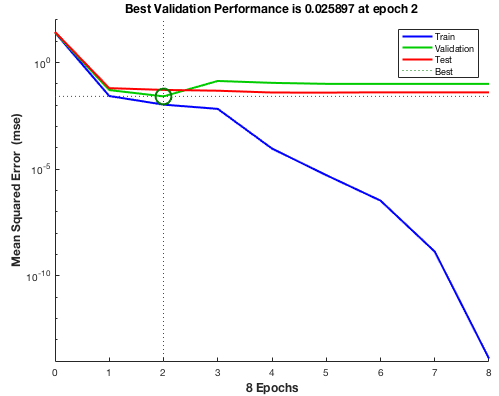
\includegraphics[width=1\linewidth]{./lab1/overfit_stop.png}
      \caption{Validation set avoids overfitting}
      \label{fig:perfect_fit}
    \end{subfigure}
    \begin{subfigure}[t]{0.3\linewidth}
      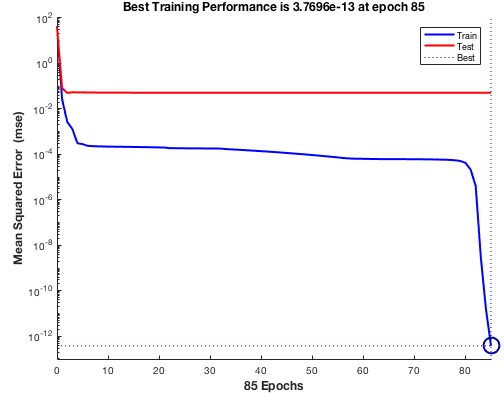
\includegraphics[width=1\linewidth]{./lab1/overfit.png}
      \caption{Overfit. 120 Neurons}
      \label{fig:overfit}
    \end{subfigure}
    \begin{subfigure}[t]{0.3\linewidth}
      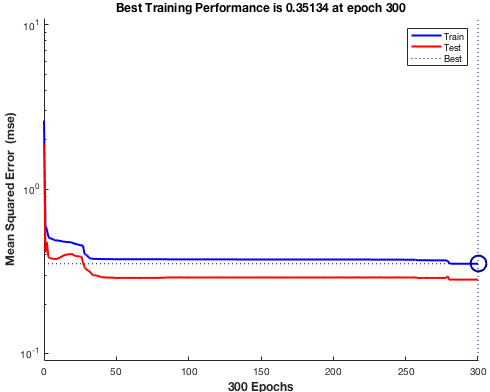
\includegraphics[width=1\linewidth]{./lab1/underfit.png}
      \caption{Underfit. 5 Neurons}
      \label{fig:underfit}
    \end{subfigure}
    \end{adjustwidth}
    \caption{Evolution of test (red), train (blue) and validation (green) set 
      MSE during training.  Left figure uses a validation set that stops befor
      e overfitting.  Otherwise, train error keeps sinking after the optima, a
      s \autoref{fig:overfit} also shows. On the right, with 5 neurons, the 
      training never converges: the net is too simple to learn the function, 
      error never decays. Test error (red) is lower than training error, it
      underfits.}
    \label{fig:validation}
  \end{figure}


  The goal here is comparing the six algorithms for training Neural Nets on
  the Matlab toolbox. For this purpose, I have trained a net using each 
  algorithm with different number of hidden units. Then, I have evaluated
  is performance on the test set, and repeated the process twenty times. 
  \autoref{tab:train_algs} shows the results of these experiments, averaged for
  each algorithm and neuron setting. Overall, all algorithms perform best
  with 80 hidden units: nets with neurons over that threshold 
  are overparametrized, since their MSE on the test set starts to decrease. 
  If there was no validation set, for 100 and 120 neurons the MSE on 
  train set would be way lower than that of test set, as
  \autoref{fig:overfit} shows. On the other hand, nets with few hidden units
  do not even learn the model, and can have higher train error than test, as in
  \autoref{fig:underfit}.

  The best algorithm
  in terms of speed and performance is the \emph{Levenberg-Marquardt} (lm)
  algorithm: it trains the fastest and it reaches better performance
  than the other ones under the same configurations. \emph{Gradient descent}
  is by far the worst, both in speed and accuracy. %The reason is that [maybe 
  %that looks for the best option/not optimized -check]

  \subsubsection{Noisy data}
    \begin{figure}[h]
      \begin{adjustwidth}{-1.1cm}{-1.1cm}
      \centering
      \begin{subfigure}[t]{0.31\linewidth}
        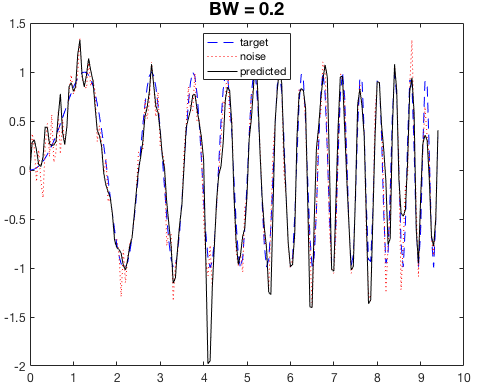
\includegraphics[width=1\linewidth]{./lab1/noise_2e-1.png}
        \caption{$R_t=0.54$, $MSE_t=0.53$}
        \label{fig:noise_small}
      \end{subfigure}
      \begin{subfigure}[t]{0.30\linewidth}
        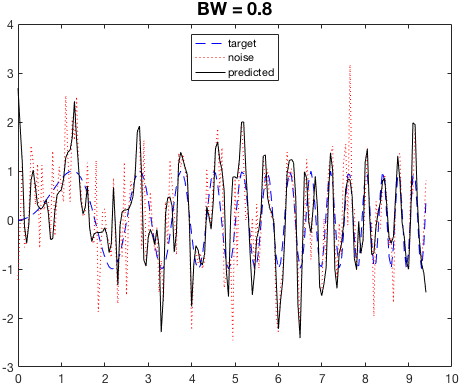
\includegraphics[width=1\linewidth]{./lab1/noise_8e-1.png}
        \caption{$R_t=0.38$, $MSE_t=2.25$}
        \label{fig:noise_big}
      \end{subfigure}
      \begin{subfigure}[t]{0.3\linewidth}
        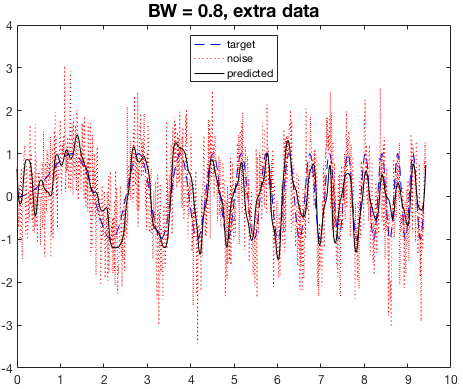
\includegraphics[width=1\linewidth]{./lab1/noise_8e-1_extra.png}
        \caption{$R_t=0.58$, $MSE_t=0.82$}
        \label{fig:noise_more_data}
      \end{subfigure}
      \end{adjustwidth}
      \caption{Estimation of a function with Gaussian noise, 0 mean, and different
        $\sigma$, or \emph{BW}. Figures (a) and (b) estimate on 190 data points, 
        figure (c) estimates on 950, 5 times more points. The network contains 80 
        hidden units, and it was trained using the \emph{lm} algorithm. MSE 
        with noisy data is worse, compared with the same setup on 
        \autoref{tab:train_algs}. Increasing the data points reduces again the 
        error, as (c) shows.}
      \label{fig:noise}
    \end{figure}

    \autoref{fig:noise} demonstrates that adding noise to the function affects
    the network estimation. It basically increases its error, no matter its
    setup. In this case, having more data points makes error go back to its
    original result: \autoref{fig:noise_more_data} shows it. This result 
    showcases another property of neural networks: they handle noisy data better
    than other estimators and even better when there is even more data, without
    increasing the demand for memory (opposed to SVM, where more data points mean
    bigger Kernel matrices).
      

  \subsection{Bayesian Inference}
  \begin{table}[h]
    \centering
    \hfill
    \begin{tabular}{@{}lrrrrr@{}}
      \toprule
      \multicolumn{6}{c}{\textbf{Levenberg-Marquardt}} \\
    N  &   $R_{t}$  &  $MSE_{t}$ &  $MSE_{tr}$ & Epch  & T(s)\\
      \midrule
      50   &   0.97    &   0.03    &  \num{0.81d-2}  &  8   &  0.15  \\
      100  &   0.90    &   0.10    &  \num{0.29d-2}  &  6   &  0.33  \\
      150  &   0.76    &   0.28    &  \num{0.01d-2}  &  5   &  0.31  \\
      300  &   0.41    &   1.00    &  \num{0.27d-2}  &  3   &  1.28  \\
      \bottomrule
    \end{tabular} 
    \hfill
    \begin{tabular}{@{}lrrrrr@{}}
      \toprule
      \multicolumn{6}{c}{\textbf{Bayesian Optimization}} \\
      N  &   $R_{t}$  &  $MSE_{t}$ & $MSE_{tr}$  & Epch  & T(s)\\
      \midrule
      50   &   1.00    &   \num{d-4}  &  \num{0.94d-7}   & 150   &    2.11  \\
      100  &   0.98    &   0.02       &  \num{0.50d-2}   & 106   &    6.52  \\
      150  &   0.89    &   0.11       &  \num{0.22d-4}   &  33   &   13.69  \\
      300  &   0.61    &   0.62       &  \num{0.19d-7}   &  27   &   92.65  \\
      \bottomrule
    \end{tabular}  \hfill\mbox{}
    \caption{Comparison between the Levenberg-Marquardt algorithm and Bayesian
    optimization, using overparametrized networks. $t$ stands for test set, $tr$
    stands for training set. As the hidden units increase, the \texttt{trainlm} 
    algorithm starts to overparametrize: validation set makes training finish 
    earlier and error on the test set increases too, whereas \emph{MSE} on the 
    training set remains constant. On the other hand, Bayes prior tries to keep
    the weights small, so test error increase is not as steep. In exchange, training
    takes more time, because finding the probabilities of each model takes
    much time.}
    \label{tab:bayes}
    \end{table}

    \autoref{tab:bayes} compares the performance of Bayesian learning against the 
    best performing algorithm from the previous section. The table showcases the
    main advantage of Bayesian optimization: it minimizes the weights of the
    network thanks to its prior distribution. Therefore, performance is better
    when there are too many hidden units. It comes at a price: training is way slower
    because there is no validation set; it calculates the probability distribution
    of the prior and the posterior at each level, which takes more time than regular
    backpropagation. The table also shows a common problem when searching the best
    parameter configuration: the \texttt{trainlm} algorithm reached its peak 
    performance with 50 neurons, but I skipped this setup on \autoref{tab:train_algs}




  





\newpage
\section{Lab 2}
  \subsection{Hopfield Network}
  Hopfield networks are recurrent NN with binary valued units that can store
  pattern according to the principles of associative memory, regarding storage
  capacity and retrieval. In this section I will illustrate their behaviour using
  them to retrieve original digits from noisy samples.

  First, the network receives an input consisting on the initial attractors. 
  In this case, the attractors are 9 handwritten digits, scanned as $15\times14$
  pixel images. So, the network has 240 features, as many as the attractors.
  The network can store up to $N / (4 \times log(N))$ patterns, $N = 240$. That
  result is 10.86, so the net should be able to store all of them without
  getting spurious patterns.
  \begin{figure}[h]
    \centering
    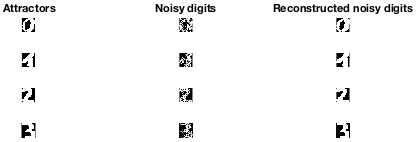
\includegraphics[width=0.6\linewidth]{lab2/digits/n1i20.png}
    \caption{Retrieved digits after 10 iterations, using a noise factor of 1. 
    Reconstruction is perfect, all patterns are retrieved}
    \label{fig:l2_no_noise}
  \end{figure}

  \begin{figure}[h]
    \centering
    \begin{subfigure}[c]{0.07\linewidth}
      
\includegraphics[width=\linewidth,height=6.1cm]{lab2/digits/noisy.png}
      \caption{Nois}
    \end{subfigure}
    \hfill
    \begin{subfigure}[c]{0.07\linewidth}
      
\includegraphics[width=\linewidth,height=6cm]{lab2/digits/col_n10i10.png}
      \caption{10}
    \end{subfigure}
    \hfill
    \begin{subfigure}[c]{0.07\linewidth}
      
\includegraphics[width=\linewidth,height=6cm]{lab2/digits/col_n10i20.png}
      \caption{20}
    \end{subfigure}
    \hfill
    \begin{subfigure}[c]{0.07\linewidth}
      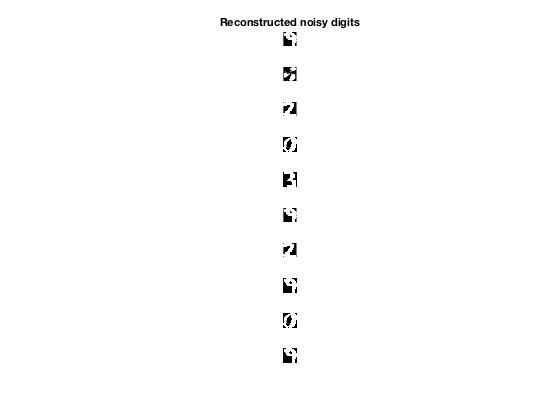
\includegraphics[width=\linewidth,height=6cm]{lab2/digits/col_n10i30.png}
      \caption{30}
    \end{subfigure}
    \hfill
    \begin{subfigure}[c]{0.07\linewidth}
      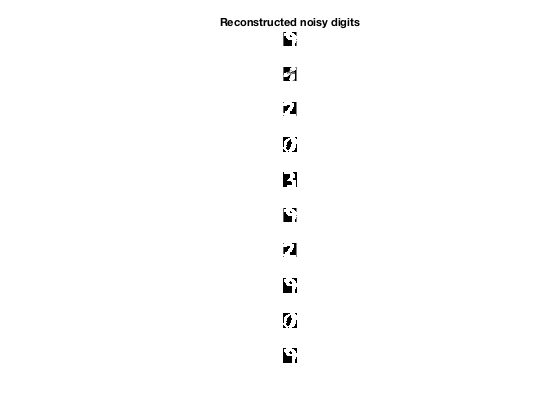
\includegraphics[width=\linewidth,height=6cm]{lab2/digits/col_n10i40.png}
      \caption{40}
    \end{subfigure}
    \hfill
    \begin{subfigure}[c]{0.07\linewidth}
      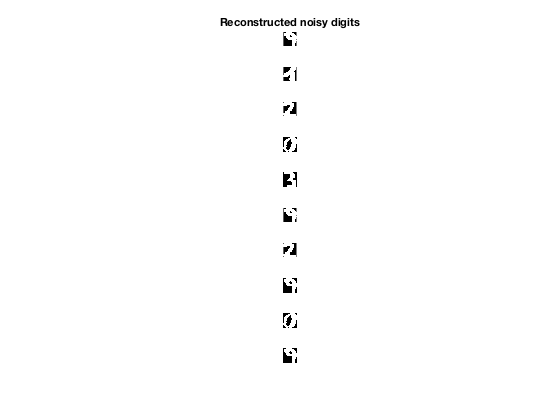
\includegraphics[width=\linewidth,height=6cm]{lab2/digits/col_n10i50.png}
      \caption{50}
    \end{subfigure}
    \caption{Retrieval process of the Hopfield network, varying the number
      of iterations, in the subcaptions. Noise factor is 10. 
      At first the network has not reached
      any minima, so it delivers noisy digits. As it keeps iterating, it approaches
      the final state. Here all original attractors are memorized, but noise is so 
      strong that the network can retrieve the wrong pattern.}
    \label{fig:l2_noisy}
  \end{figure}

  Indeed, no spurious pattern is retrieved. With low noise, as in 
  \autoref{fig:l2_no_noise}, reconstruction is perfect even after 10 iterations,
  and it remains stable afterwards (low \emph{crosstalk}). On 
  \autoref{fig:l2_noisy} noise is way higher. It takes more time to converge,
  so the digits retrieved during the first 40 iterations still have some noise,
  equilibrium is only reached after 50 epochs.
  Furthermore, corruption has pulled the data points too close to the 
  wrong attractors,
  so the wrong digit is commonly retrieved. But, as dimensionality is so high,
  all patterns are properly stored, and there is no convergence on spurious, 
  local minima. 

  \subsection{Elman network}
  Elman networks are a kind of Recurrent Neural Networks, were the output is
  fed to the input for the following training/simulation step. Therefore, they
  can learn temporal patterns from data, and they are often used for time series
  prediction.

  I have tested the network on the \emph{Hammersteim system} data using
  different configurations. First, I have tuned the training set size:
  I have used 100, 200, 300 and 500 datapoints under the default configurations
  (50 neurons, 500 training epochs), and they have delivered 0.41, 0.30, 0.22 and
  0.07 MSE on the test set, respectively. So, the network performance improves
  as it has more data points, similarly to other kind of networks.

  
  Increasing the neurons (beyond 50) decreases performance: testing with 50, 100,
  150 and 250 I have obtained MSE of 0.14, 1.52, 2.20 and 3.78 respectively.
  50 is already good; more than that overparametrizes the network.

  I also also have tried different architectures and training epochs, shown in 
  \autoref{tab:l2_elman_transfers}. As expected, the second layer should
  use a linear activation function: having non linear activation functions on
  the last layer pushes prediction values towards 1 and -1. Of the both 
  tested functions, the hyperbolic tangent works best. Increasing epochs
  improves performance until they exceed 100; particularly on the \texttt{purelin}
  function. This means that the network is overfitting beyond that point.

  Finally, I am showing the result of training and testing the network using
  an optimal configuration in \autoref{fig:l2_optimal_elman}.


  \begin{table}
    % this is a lie: it was th eother way around
    \centering
    \begin{tabular}{@{}llrrrr@{}}
      \toprule
      2nd layer& 1st layer& 10 & 50 & 100 & 500 \\
      \midrule % using 'tansig' second
      \multirow{2}{*}{\texttt{purelin}} & \texttt{tansig}  & 1.05  &  0.32  &
                                                             0.27  &  0.38 \\
      & \texttt{logisg}  & 0.97  &  0.92  &  0.31  &  0.43 \\
      \bottomrule
    \end{tabular}
    \hfill
    \begin{tabular}{@{}lllrrrr@{}}
      \toprule
      2nd layer& 1st layer& 10 & 50 & 100 & 500 \\
      \midrule % using 'tansig' second
      \multirow{2}{*}{\texttt{tansig}} & \texttt{tansig}  & 44.46 &  1.57  &
                                                             2.81  &  0.71 \\
      & \texttt{logisg}  & 1.35  &  0.95  &  0.92  &  1.26 \\
      \bottomrule
    \end{tabular}
    \caption{MSE for different combinations of training epochs and training
    functions. The best architecture seems to be having a \texttt{purelin} 
    architecture on the second layer, and a \texttt{logsig} on the second. All
    nets had 50 neurons, and were trained using 500 datapoints. The shown results
    have been averaged over 20 experiments}
    \label{tab:l2_elman_transfers}
  \end{table}

  \begin{figure}[htpb]
    \centering
    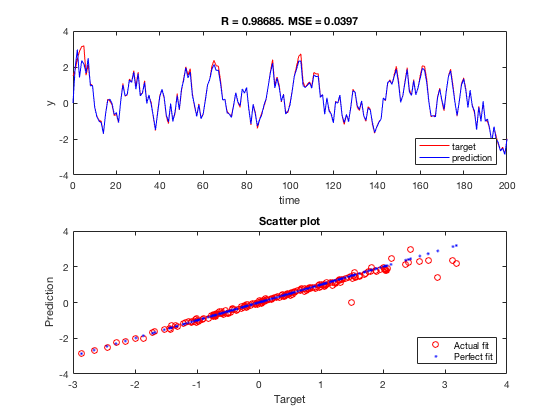
\includegraphics[width=0.8\linewidth]{lab2/elman_optimal.png}
    \caption{Test set function estimation on the \emph{Hammersteim system}, using
    the optimal parameter configuration from the previous experiments: 50 hidden
    units, 100 epochs, an hyperbolic tangent transfer function on the first layer,
    a linear function on the second and 500 points for training.}
    \label{fig:l2_optimal_elman}
  \end{figure}


  \newpage
\section{Lab 3: Unsupervised Learning}
  \subsection{Principal Component Analysis}
  \begin{figure}[h]
    \begin{adjustwidth}{-1cm}{-1cm}
    \centering
    \begin{subfigure}[t]{0.3\linewidth}
      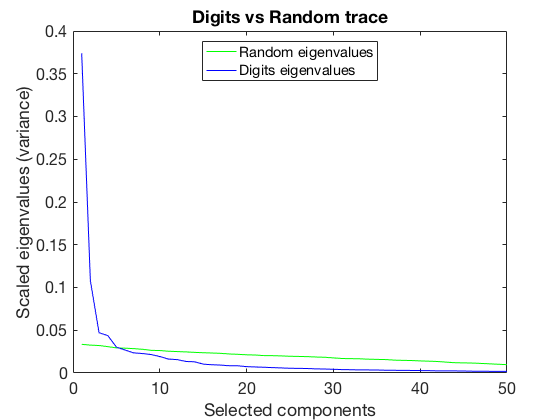
\includegraphics[width=1\linewidth, height=4.4cm]{./lab3/PCA/digits_vs_random_trace.png}
      \caption{Eigenvalues by PC}
      \label{fig:l3_traces}
    \end{subfigure}
    \begin{subfigure}[t]{0.29\linewidth}
      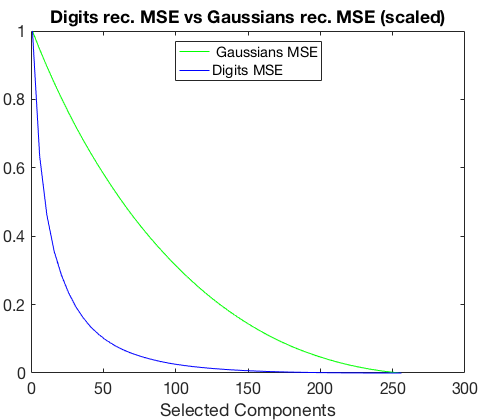
\includegraphics[width=1\linewidth, height=4.4cm]{./lab3/PCA/digits_vs_random_recMSE.png}
      \caption{Rec. \emph{MSE} by PC (scaled)}
      \label{fig:l3_rec_MSE}
    \end{subfigure}
    \begin{subfigure}[t]{0.3\linewidth}
      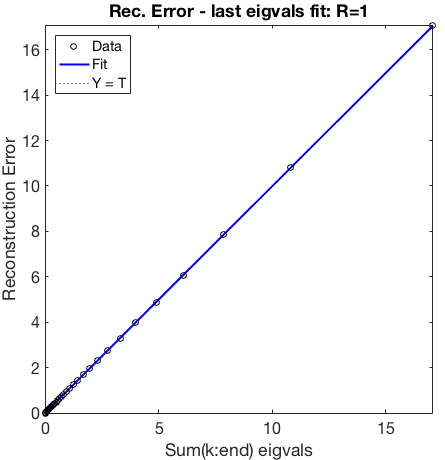
\includegraphics[width=1\linewidth, height=4.3cm]{./lab3/PCA/regression.png}
      \caption{Lin. fit: MSE and left-out variance}
      \label{fig:l3_regression}
    \end{subfigure}
    \end{adjustwidth}
    \caption{Comparison between a synthetic dataset (green) and the 
      \emph{threes} dataset, using their eigenvalues by PC (left) and their
      reconstruction error (centre, scaled by their max. value).
      Right image shows a perfect linear relation between recovery error and
      the summed variance of all the components but the first $k$ ones.}
    \label{fig:l3_first_task}
  \end{figure}

  The goal of this section is to understand the meaning and consequences of using
  PCA. \autoref{fig:l3_first_task} compares its behaviour on the \emph{threes} 
  dataset and on a random dataset of 256 I.d. Gaussian features. For the 
  \emph{threes} most information lies on the first PC: according to
  \autoref{fig:l3_traces}, 50 components explain already 90\% of the variance. On
  the Gaussians, that makes less than 40\%. Therefore, 50 components 
  should already deliver a good reconstruction of the digits, as 
  \autoref{fig:l3_rec_MSE} shows: MSE decreases steeply until then, and slowly 
  afterwards. On the other hand, on the Gaussian dataset information is 
  distributed evenly among the components. Both eigenvalues and MSE do not 
  decrease so sharply, there is no optimal transformation of the data such 
  that more information lies on a specific direction. 

  \begin{figure}[h]
    \centering
    \hfill
    \begin{subfigure}[t]{0.4\linewidth}
      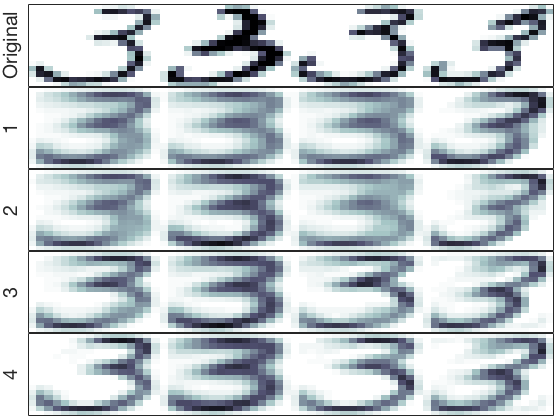
\includegraphics[width=\linewidth, height=4.3cm]{./lab3/PCA/mosaics/PC_1_4_small.png}
      %\caption{Few PC. $MSE(rec) > 0.9; variance < 12\%$}
      \label{fig:few_pc}
    \end{subfigure}
    \hfill
    \begin{subfigure}[t]{0.4\linewidth}
      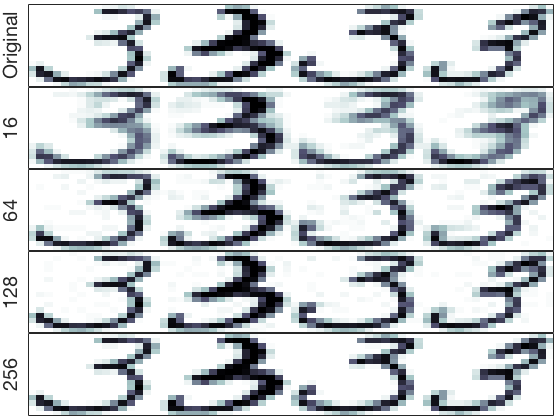
\includegraphics[width=\linewidth,height=4.3cm]{./lab3/PCA/mosaics/PC_16_256_small.png}
      %\caption{Many PC. $MSE(rec) < 0.75; variance > 45\%$}
      \label{fig:many_pc}
    \end{subfigure}
    \hfill \mbox{}
    \caption{Reconstruction of four different samples (columns) with increasing
      number of components (rows). Top row of each table contains the 
    original samples. Vertical labels indicate the number of components}
    \label{fig:l3_threes_pc}
  \end{figure}

  \paragraph{Visual reconstruction} a sample with few components 
  if much different from the original image, as the images on 
  \autoref{fig:l3_threes_pc} show. These recovered images seem more similar 
  to the average three. %TODO: put average three somewhere
  The reason is that the first components model the main structure underlying 
  all the data, the \emph{essence} of the \emph{threes}.
  As more components are added, reconstruction becomes more accurate.  The last 
  components model the noise, the particularities of each data point. Since
  most variance lies below 50 PC, any reconstruction with more PC delivers
  almost the same result, there is little margin of improvement. 
  With 256 PC the recovered image is exactly the same, and the \emph{MSE} is 0.
  %% maybe remove this
  There is a mathematical proof: being data $X \in {\rm I\!R}^{d \times N}$,
  with $d$ the input feature space; $V \in {\rm I\!R}^{d \times s}$ the
  eigenvector matrix, $s$ selected components; and $X_s=V^{t}X$ the data
  projected on those components. If $s=d$, then $VV^{t}=I$ (full rank orthogonal matrix).
  Then, $\hat{X} = VX_s = VV^{t}X = X$. 
  
  \begin{figure}[h]
    \centering
    \hfill
    \begin{subfigure}[t]{0.15\linewidth}
      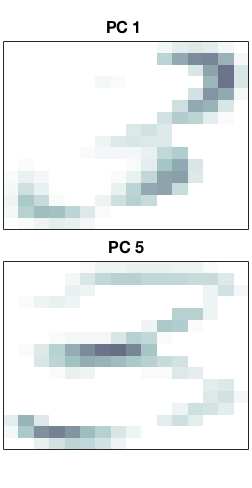
\includegraphics[width=\linewidth, height=5.5cm]{./lab3/PCA/PC_interpret/PC1+PC5.png}
    \end{subfigure}
    \hfill
    \begin{subfigure}[t]{5.4cm}
      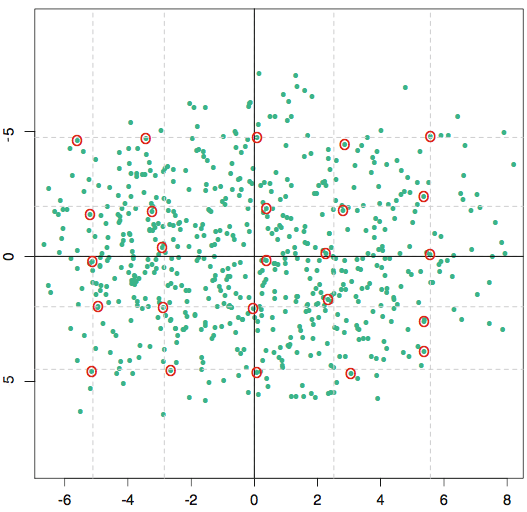
\includegraphics[width=\linewidth, height= 5.1cm]{./lab3/PCA/PC_interpret/quantiles.png}
    \end{subfigure}
    \hfill
    \begin{subfigure}[t]{5.4cm}
      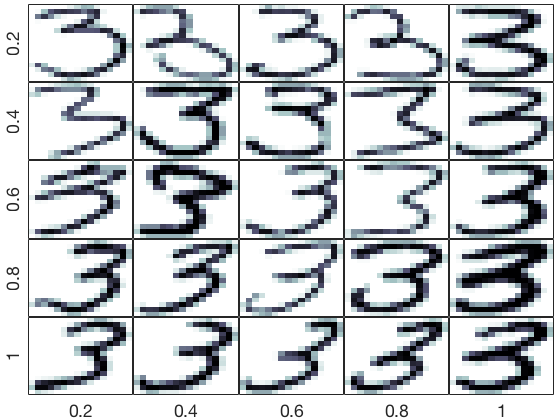
\includegraphics[width=\linewidth, height = 5.0cm]{./lab3/PCA/PC_interpret/Y1_X5.png}
    \end{subfigure}
    \hfill \mbox{}
    \caption{1st and 5th PC (left), and data points when projected on them 
    (centre). X axis correspond to the fifth, Y to the first. Red dots 
    show the closest data point to a quantile on the projections distribution.
    These samples are shown on the right image, with their corresponding quantile.}
    \label{fig:l3_pc_interpret}
  \end{figure}
  
  \paragraph{Component interpretation} each PC models data particularities, that
  can be used to find patterns on it, and even for clustering. 
  \autoref{fig:l3_pc_interpret} shows a representation of the first and fifth 
  component. Then, I have taken the points corresponding to different quantiles
  of the data, when projected on those components. The results are shown on the
  right image. PC 1 models cursiveness: threes on the Y axis lean to the left
  side on the low quantiles (top), and become totally cursive on the bottom rows.
  The fifth (X axis) models thickness on the horizontal strokes: digits at the 
  highest quantile (quantile) are the thickest.

  
  \subsection{Self Organizing Maps}
  %https://nl.mathworks.com/help/nnet/ug/cluster-with-self-organizing-map-neural-network.html
  \begin{figure}[h]
    \begin{adjustwidth}{-1cm}{-1cm}
    \centering
    \begin{subfigure}[t]{0.32\linewidth}
      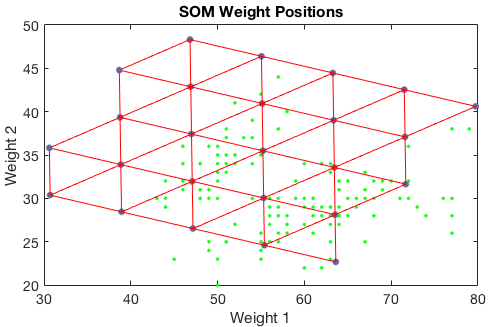
\includegraphics[width=1\linewidth]{./lab3/SOM/init_hex.png}
      \caption{Network initialization.}
      \label{fig:l3_init}
    \end{subfigure}
    \begin{subfigure}[t]{0.31\linewidth}
      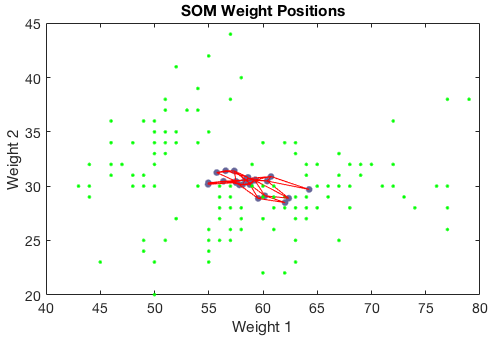
\includegraphics[width=1\linewidth]{./lab3/SOM/epoch1_hex.png}
      \caption{Training after one epoch}
      \label{fig:l3_epoch1}
    \end{subfigure}
    \begin{subfigure}[t]{0.31\linewidth}
      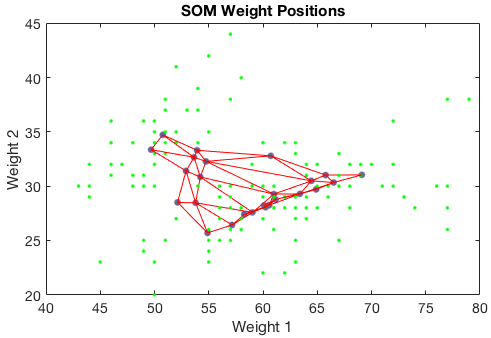
\includegraphics[width=1\linewidth]{./lab3/SOM/epoch5_hex.png}
      \caption{Final result}
      \label{fig:l3_epoch5}
    \end{subfigure}
    \end{adjustwidth}
    \caption{Training state evolution of a SOM with 25 neurons, set in a 
    hexagonal grid of $5\times5$. On the first epoch, many neurons
    are pulled together into the regions of high variance, since their 
    neighbourhood radius is very large. At later stages, neighbourhood size 
    shrinks and less neurons are pulled from their position.}
    \label{fig:l3_hex_grid}
  \end{figure}

  SOM deliver meaningful representations of the data (vector quantization) using
  competitive learning to make their neurons learn the data distribution. 
  Basically, as a neuron “wins” over the others for a data point, its weight is
  updated so it is closer to the input, according to the Konohen rule. 
  The new state depends on both the previous state and the input, and each
  has a different weight (parameter $\alpha$). Besides, neurons also pull their
  neighbours, defined by a radius on some distance metric and grid disposition. 
  \autoref{fig:l3_hex_grid} showcases the learning process of the SOM. Furthermore,
  they can also be used for clustering, with as many clusters as neurons. 
  \autoref{tab:l3_som_grid} compares clustering performance with different 
  configurations, using 3 clusters.

  \begin{table}[h]
    \centering
    \begin{tabular}{@{}llrrrrrrr@{}}
      \toprule
      & \phantom{ab}  & \texttt{linkdist} & \phantom{ab} & \texttt{dist} & 
      \phantom{ab} & \texttt{boxdist} & \phantom{ab} & \texttt{mandist} \\
      \midrule
      \textbf{Hexagonal} &&  $0.7240$  &&   $0.7240$  &&   $0.7254$  &&  $0.7239$\\
      \textbf{Grid}      &&  $0.7254$  &&   $0.7233$  &&   $0.7247$  &&  $0.7226$\\
      \textbf{Random}    &&  $0.6817$  &&   $0.7240$  &&   $0.7246$  &&  $0.7240$\\
      \bottomrule
    \end{tabular} 
    \caption{Comparison of different topologies and distances for the iris dataset,
    using a $3 \times 1$ network for clustering. The displayed numbers correspond 
  to the ARI index.}
    \label{tab:l3_som_grid}
  \end{table}

\section{Lab 4}
  \subsection{Stacked autoencoders}
  \begin{table}[h]
    \centering
    \begin{tabular}{@{}lrrrrr@{}}
      \toprule
      && \multicolumn {2}{c}{Accuracy on Autoencoder} \\
      \cmidrule{3-4} 
      Layers & Hidden units & Before tuning & After tuning & 
      Regular net accuracy & \textbf{Improvement} \\
      \midrule
      2   & [100]           &  98.38   &  98.92  &   97.60  &  \textbf{1.35}\% \\
      3   & [100 81]        &  78.82   &  99.92  &   96.68  &  \textbf{3.35}\% \\
      4   & [100 81 64]     &  38.22   &  99.78  &   96.92  &  \textbf{2.97}\% \\
      5   & [100 81 64 49]  &  21.50   &  99.40  &   97.58  &  \textbf{1.87}\% \\
      \bottomrule
    \end{tabular} 
    \caption{Evaluation of different deep architectures. \emph{Hidden layers} 
    indicates the neurons on each layer (from the first to the last), on both
    the autoencoders and the regular feed forward net. The final column shows
    the improvement of the stacked architecture over the feed forward net,
    in digits classification. For each row, both type of nets share the same
    structure}
    \label{tab:l4_autoencoders}
  \end{table}
  % maybe remove this
  \begin{figure}[htpb]
    \centering
    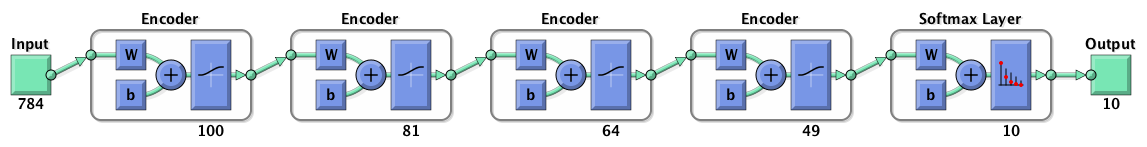
\includegraphics[width=\linewidth]{lab4/deep_architecture.png}
    \caption{5 layer architecture of autoencoders, corresponding to last row
    of \autoref{tab:l4_autoencoders}}
    \label{fig:l4_architecture}
  \end{figure}

  The goal of this section is understanding the behaviour of autoencoders, 
  regarding their performance compared to regular nets, as well as interpreting
  what they do. 

  \autoref{tab:l4_autoencoders} shows that autoencoders outperform regular deep
  feedforward networks, even when sharing the same structure. Furthermore, 
  they offer a more efficient representation of data, which could eventually
  used to save storage space. The main drawback is the time that
  the layerwise greedy training takes, compared to training a simple 
  network using backpropagation. Also, fine tuning makes a big difference in 
  performance, particularly for deeper architectures. It is not good to skip it.
  Very large architectures are usually trained using GPUs.

  \begin{figure}[htpb]
    \centering
    
\includegraphics[width=\linewidth]{lab4/layer_features.png}
    \caption{Original digit (left), and the features that each autoencoders 
      extracts from it, using the 5 level deep architecture of 
      \autoref{tab:l4_autoencoders}. As depth increases,
      features become more abstract and hard to understand for humans. Also,
      their dimensionality is reduced (less pixels on the image). From left to
      right, images correspond to autoencoders 1 to 4.}
    \label{fig:l4_features}
  \end{figure}

  Stacked autoencoders extract abstract features from data, in a similar way
  the brain does. The deeper the architecture, the more abstract features become.
  \autoref{fig:l4_features} showcases this idea: the features, represented as 
  images, that each layer obtains have no meaning for an human. This is actually
  one of the main problems of deep learning: they often produce \emph{black box}
  models, and we cannot understand what it actually represents. Therefore, they
  cannot be used at applications that require transparency, like credit scoring.
  However, this abstraction is their main advantage: as I showed in the previous
  paragraph, it beats regular nets with the same structure. 

  \begin{figure}[htb]
    \centering
    \hfill
    \begin{subfigure}[t]{0.25\linewidth}
      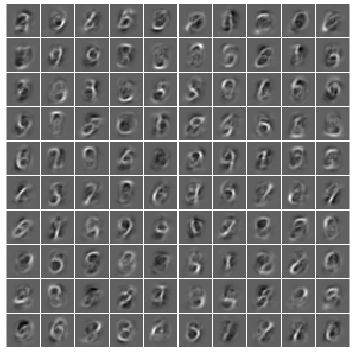
\includegraphics[width=1\linewidth]{lab4/weights_default.png}
      \caption{$L2\ weight = 2 \times 10^{-3}$}
    \end{subfigure}
    \hfill
    \begin{subfigure}[t]{0.245\linewidth}
      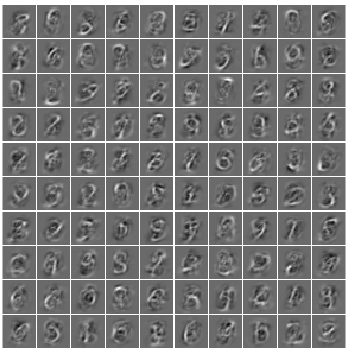
\includegraphics[width=1\linewidth]{lab4/weights_regulariz1e-3.png}
      \caption{$L2\ weight = 1 \times 10^{-3}$}
    \end{subfigure}
    \hfill
    \begin{subfigure}[t]{0.25\linewidth}
      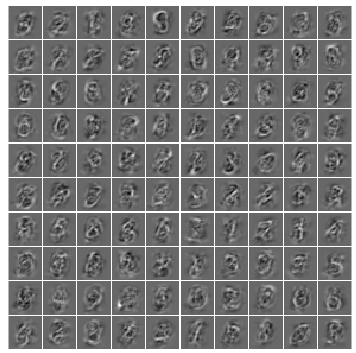
\includegraphics[width=1\linewidth]{lab4/weights_regulariz5e-4.png}
      \caption{$L2\ weight = 5 \times 10^{-4}$}
    \end{subfigure}
    \hfill \mbox{}
    \caption{Weights of the first autoencoder. This plot is very analogous
    to that of the components in \autoref{fig:l3_pc_interpret}: it displays
    the internal abstract representation the data, but using weights instead of 
    components.  
    Each image is the result of a different L2 regularization weight. }
    \label{fig:l4_weights}
  \end{figure}

  Finally, \autoref{fig:l4_weights} shows the weights of the first layer after
  training with different L2 penalties. Higher penalties make the model simpler,
  so weights are more similar to actual digits. Lower penalties make weights
  have a higher variance (the model is more complex), therefore they look
  blurrier on the right image. This
  is analogous to the ideas I explored in the previous section, particularly 
  on \autoref{fig:l3_pc_interpret}: each weight, or component in the case of 
  PCA, model different characteristics of the data (cursiveness, thickness, 
  etc.). This is also one of the reasons for the popularity of deep neural 
  networks: they perform automatic and parametrized feature extraction and 
  selection.

  \subsection{Convolutional Neural Networks}
  The \texttt{CNNEx.m} script runs a convolutional net on a database with images
  of laptops, trains and boats, and tries to classify them, as well as show their
  internal representation. The dimension of the weights in layer 2 is [11 11 3 
  96],  with stride [4 4] and no padding. This is the convolutional filtering 
  layer.  The stride is the step size for 
  traversing the input vertically and horizontally. In this case, [4 4] 
  specifies a vertical step size of 4 and a horizontal step size of 4.
  The first two numbers are the filter size (11x11):  width and height 
  to scan the image, 121 pixels in total. The third number (3) is the number 
  of channels. The image is coloured, so they are the RGB channels. 
  The last number, 96, is the number of filters, I.e  the number of neurons 
  that corresponds to a region of the output.  

  On the second question, the fifth layer performs Pooling, using a stride of
  [2 2] and a filter size of  [3 3], with no padding. Starting on the first 
  layer, the input is $227 \times 227$.
  The output after first convolution is $(Size - Filter + 2 \times Paddding)/
  stride + 1$. So: $(227 - 11) / 4 + 1 = 55$, so there are $55 \times 55$ 
  neurons. They go then through the pooling layer, 
  obtaining $(55 - 3)/2 + 1 = 27$, so layer 6 expects an input of $27 \times 27$.

  Applying this iteratively returns that on the last layer there are
  $71 \times 71$ feature maps, so 5041 neurons. After the first layer there 
  were $11 \times 11 \times 3 \times 96 =34848$, which is a big improvement.
  \newpage

\section{Final project}
My name is Mauro Paradela del Río, student number r0696150, Master in Artificial
Intelligence. My data has been generated using:

$$ Tnew = (9T1 + 6T2 + 6T3 + 5T4 + 1T5) / (9 + 6 + 6+ 5 + 1) $$

  \subsection{Regression}
  For this exercise I have to estimate a function generated using my student
  number, using the formula above. The result of this operation is a combination
  of non linear functions, that is also non linear. The result is plotted in 
  \autoref{fig:project_dataset}.
  \begin{figure}[htb]
    \centering
    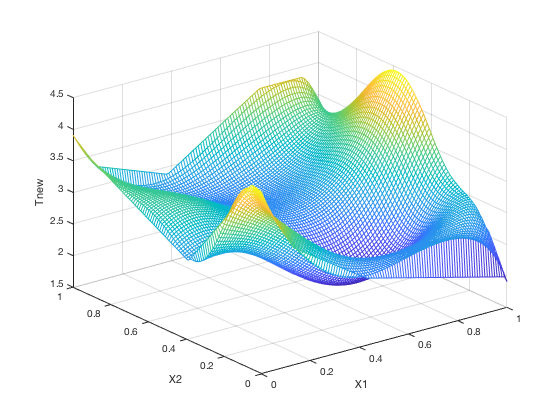
\includegraphics[width=0.5\linewidth]{project/dataset.png}
    \caption{Function produced using my student number}
    \label{fig:project_dataset}
  \end{figure}
  \begin{table}[h!]
    \begin{tabular}{@{}lrrrrr@{}}
      \toprule
      \multicolumn{5}{c}{\textbf{tansig}} \\
      N  &   $R_t$  &  $MSE_t$ & $MSE_{tr}$ &  Epch  & T(s)\\
      \midrule
      25   & 0.99   &   \num{9.79e-05}  & \num{2.39e-05}  &  169  &  11.08 \\
      50   & 0.99   &   \num{1.67e-05}  & \num{6.90e-06}  &  171  &  10.64 \\
      100  & 0.99   &   \num{1.05e-05}  & \num{1.34e-06}  &  200  &  20.15 \\
      150  & 0.99   &   \num{2.73e-06}  & \num{8.29e-07}  &  200  &  16.54 \\
      200  & 0.99   &   \num{5.38e-06}  & \num{1.71e-06}  &  200  &  12.55 \\
      250  & 0.99   &   \num{1.40e-05}  & \num{3.42e-06}  &  200  &  12.49 \\
      300  & 0.99   &   \num{1.35e-05}  & \num{2.29e-06}  &  198  &  12.54 \\
      \bottomrule
    \end{tabular} 
    \hfill
    \begin{tabular}{@{}rrrrr@{}}
      \toprule
      \multicolumn{5}{c}{\textbf{logsig}} \\
      $R_t$  &  $MSE_t$ & $MSE_{tr}$ &  Epch  & T(s)\\
      \midrule
       0.99   &   \num{4.53e-06}  & \num{1.46e-06}  &  200  &  16.19 \\
       0.99   &   \num{6.11e-06}  & \num{1.50e-06}  &  200  &  16.87 \\
       0.99   &   \num{9.63e-06}  & \num{6.17e-06}  &  160  &  11.55 \\
       0.99   &   \num{1.45e-05}  & \num{4.80e-06}  &  172  &  11.96 \\
       0.99   &   \num{1.45e-04}  & \num{5.89e-06}  &  167  &  15.66 \\
       0.99   &   \num{5.07e-05}  & \num{3.24e-05}  &  165  &  12.49 \\
       0.99   &   \num{3.79e-06}  & \num{1.14e-06}  &  200  &  15.62 \\
      \bottomrule
    \end{tabular} 
    \caption{Metrics on different network configurations, always with
      one hidden layer and trained using \texttt{trainlm}. I compare two different
      transfer functions on the first layer. All results are the average
      of 20 runs.
      $N$ stands for the hidden units,$t$ stands for $test$ and
      $tr$ stands for training. It looks like any model is good for this dataset.}
    \label{fig:project_feedforward}
  \end{table}

  \autoref{fig:project_feedforward} shows a comparison of different network
  architectures, focusing particularly on the transfer function and the number
  of hidden units. For the experiments I have taken 1000 points as validation 
  set, another 1000 for training and 1000 for testing, avoiding overlapping 
  between them. Apparently, a simple network of 25 hidden units with any
  transfer function produces already a very good result: on the train set, MSE
  is below \num{1e-4}, and the correlation with that same set is above 0.99.
  The only remarkable fact is that \texttt{tansig} converges slightly faster than
  \texttt{logsig}, but error seems to be higher. \autoref{fig:l5_mse_curves}
  showcases it on the MSE curve evolution: \texttt{logisg} overcomes \texttt{tansig}
  at 50 epochs, but takes more iterations to reach its best performance. In contrast,
  The former is already semi-optimal at 20 epochs, the latter descends steeply at 30.

  I believe that the non linear structure of the function is well captured by the 
  net. Furthermore, since all values are positive, \texttt{logsig}
  approximates it very well. A way of improving the results would be training
  under Bayesian Optimization: since so few neurons are required, it is easy
  to overparametrize. Bayesian optimization would reduce overfitting in that 
  case.

  \begin{figure}[ht]
    \centering
    \begin{subfigure}[t]{0.35\linewidth}
      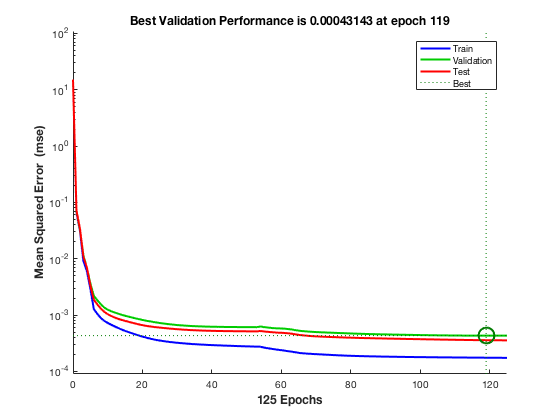
\includegraphics[width=1\linewidth]{./project/tansig_MSE.png}
      \caption{\texttt{tansig}}
    \end{subfigure}
    \begin{subfigure}[t]{0.35\linewidth}
      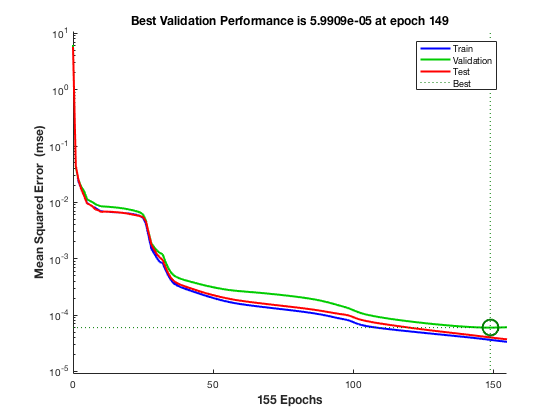
\includegraphics[width=1\linewidth]{./project/logsig_MSE.png}
      \caption{\texttt{logsig}}
    \end{subfigure}
    \caption{MSE curve on all sets, for different transfer functions on the 
    first layer. There are 25 hidden units, trained using the \texttt{trainlm}
  algorithm. Both behave differently: \texttt{tansig} converges faster, but
    \texttt{logsig} achieves better results.}
    \label{fig:l5_mse_curves}
  \end{figure}

  \begin{figure}[htb]
    \begin{adjustwidth}{-1.1cm}{-1.1cm}
    \centering
    \begin{subfigure}[t]{0.31\linewidth}
      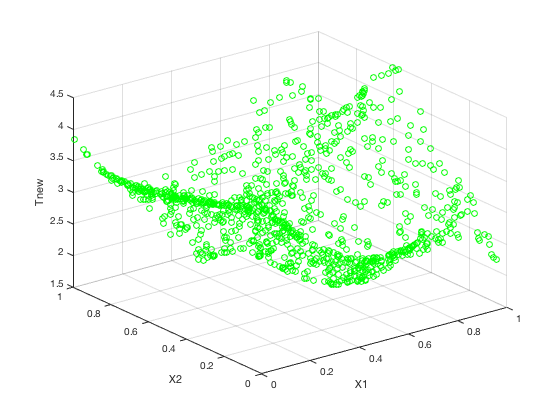
\includegraphics[width=1\linewidth]{./project/scatter_ytest_green.png}
      \caption{Test set}
    \end{subfigure}
    \begin{subfigure}[t]{0.31\linewidth}
      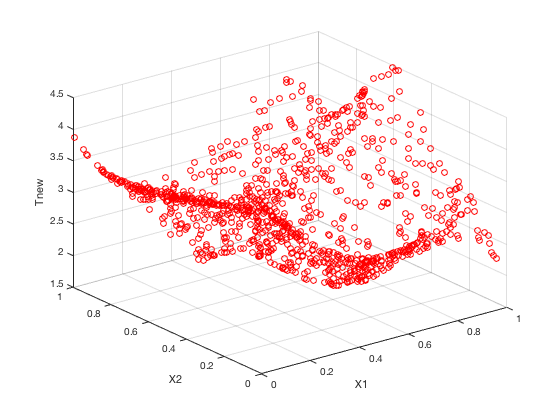
\includegraphics[width=1\linewidth]{./project/scatter_ysim.png}
      \caption{Prediction}
      \label{fig:overfit}
    \end{subfigure}
    \begin{subfigure}[t]{0.29\linewidth}
      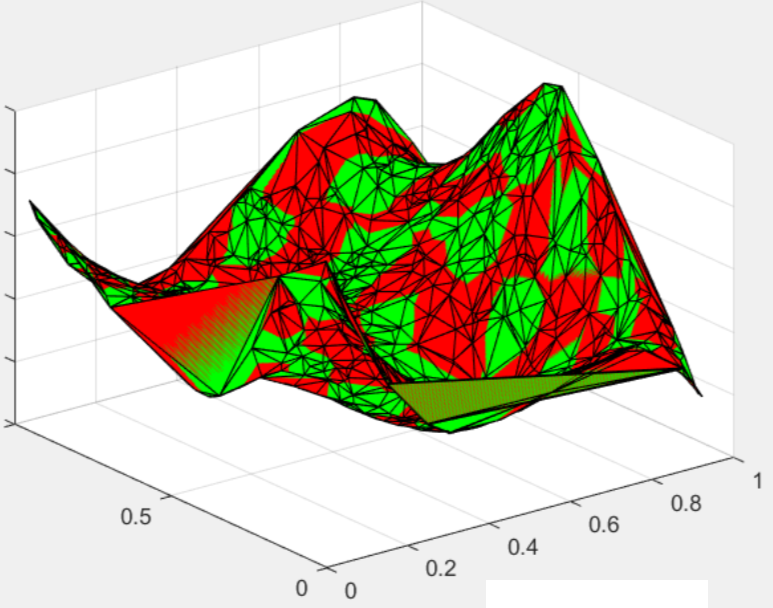
\includegraphics[width=1\linewidth]{./project/sim_and_test.png}
      \caption{Both together (interpolated)}
      \label{fig:underfit}
    \end{subfigure}
    \end{adjustwidth}
    \caption{Test set (green) and network prediction (red) comparison. 25 hidden units,
      \texttt{logsig} transfer function. MSE on this set is below \num{1e-5}}
    \label{fig:l5_regression_test}
  \end{figure}

  \subsection{Classification}
  In this part of the assignment I have to build a feed forward neural network to
  classify wine into categories. The last number of my student ID is 0, so I have
  a binary problem with 2198 data points on the negative class (label 6) and 
  1457 data points on the positive class (label 5), taken from the white wine 
  subset. 

  For this task I have focused on Matlab's \emph{patternnet}: a feed forward net
  with a \emph{softmax} function on the output layer. That way the network
  results ranges between 0 and 1 for each output neuron. When using a 
  \emph{one-hot} encoding for the classes, they can be
  interpreted as probabilities of belonging to one class or the other. Therefore,
  in this particular problem all target values are bidimensional vectors, either
  [0 1] or [1 0].

  \paragraph{Choosing the optimal architecture} On 
  \autoref{tab:l5_classif_algorithms} I have tested different training algorithms
  for pattern estimation. Some of them are new, like Scaled Conjugated Gradient
  (\emph{trainscg}) and Resilient Backpropagation (\emph{trainrp}). The results
  show once again that Levenberg-Marquardt delivers the best results. However,
  this time it is by far the slowest algorithm: it takes up to 50 times more
  then \emph{trainscg} when using 80 hidden units, for example. Even though
  it does not calculate the whole Hessian matrix, the lm is too slow
  when doing pattern classification, even though it was the best performing
  algorithm for function estimation (see \autoref{tab:train_algs}).
  The figure also shows that 5 neurons are
  enough for delivering a decent CCR, although it does not overparametrize very
  fast: the value keeps constant for the configurations I have tested.

  \begin{table}[htb]
    \resizebox{\textwidth}{!}{%
    \begin{tabular}{@{}lrrrrrrrrrrrrrrrrrrrr@{}}
    \toprule
    \multirow{2}{*}{\emph{Nhid}}&& \multicolumn{3}{c}{\textbf{trainscg}} && \multicolumn{3}{c}{\textbf{trainrp}} &&
      \multicolumn{3}{c}{\textbf{traingd}} && \multicolumn{3}{c}{\textbf{trainlm}} &&
      \multicolumn{3}{c}{\textbf{trainbfg}} \\
 && $CCR$ & $Epch$ & $T(s)$ && $CCR$ & $Epch$ & $T(s)$ && $CCR$ & $Epch$ & $T(s)$ && $CCR$ & $Epch$ & $T(s)$ && $CCR$ & $Epch$ & $T(s)$ \\
\midrule
  5 && 0.70 & 25 & 0.36 && 0.70 & 38 & 0.27 && 0.60 & 431 &  2.66 && 0.71 & 14 &  0.81 && 0.72 &  9 &  0.54 \\
 10 && 0.70 & 22 & 0.41 && 0.70 & 48 & 0.34 && 0.59 & 461 &  3.06 && 0.72 &  8 &  1.03 && 0.74 & 14 &  0.61 \\
 20 && 0.70 & 23 & 0.49 && 0.70 & 46 & 0.43 && 0.59 & 440 &  3.87 && 0.73 & 10 &  3.43 && 0.72 & 20 &  1.43 \\
 40 && 0.70 & 19 & 0.56 && 0.71 & 45 & 0.68 && 0.59 & 478 &  7.40 && 0.74 & 14 & 16.84 && 0.71 & 31 &  6.89 \\
 60 && 0.70 & 17 & 0.76 && 0.71 & 41 & 0.79 && 0.60 & 457 &  7.72 && 0.73 & 10 & 28.42 && 0.70 & 32 & 28.86 \\
 80 && 0.70 & 18 & 0.90 && 0.71 & 44 & 1.11 && 0.60 & 478 & 10.10 && 0.75 & 10 & 52.12 && 0.70 & 17 & 39.84 \\
      \bottomrule
  \end{tabular}}
  \caption{Comparing different units on the hidden layer and training methods for
  the feedforward \emph{patternnet} on the white wine dataset. This time, the
most accurate algorithm is not the fastest; quite the opposite. \emph{CCR} stands
for Correctly Classfied Data on the validation set, and \emph{Epch} for epoch 
of convergence in the training phase. Validation and test set are each 15\% of
the data points.}  
  \label{tab:l5_classif_algorithms}
  \end{table}

  \newpage
  \paragraph{Dimensionality reduction} using linear PCA has two potential benefits:
  it can save memory and computations by reducing the size of the data, and it
  can find directions in which classification can deliver better results. According
  to \autoref{fig:l5_PC}, 3 components are already a very good summarization of
  the data: they contain most (almost 100\%) of the variance, and reconstruction
  error using 3 components is almost 0. So, the first goal is achieved. However,
  classification does not improve: as \autoref{tab:l5_transfer_PC}, no combination
  of hidden units and transfer functions outperforms the results from 
  \autoref{tab:l5_classif_algorithms}, in this case for Resilient Backpropagation.
  I have even tried different transfer functions on the first layer, but accuracy
  is on all of them around 15\% lower than it was. I believe that PCA is not finding
  an optimal direction where classes can be separated well. 
  \autoref{fig:l5_wine_gmatrix} proofs it: in all the extracted 3 components 
  both classes have a large overlapping.

  I would like to point out that I have not changed the transfer function on the
  last layer (\texttt{softmax}) because it is the right one for a classification 
  task. A linear activation function would deliver values over 1 and below 0, and
  \texttt{logsig} is not suitable for multiclass problems. 

  \begin{figure}[ht]
    \centering
    \begin{subfigure}[t]{0.4\linewidth}
      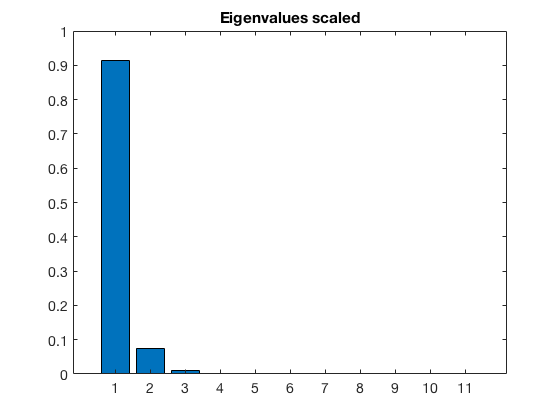
\includegraphics[width=1\linewidth]{./project/wine_eigvals.png}
    \end{subfigure}
    \begin{subfigure}[t]{0.4\linewidth}
      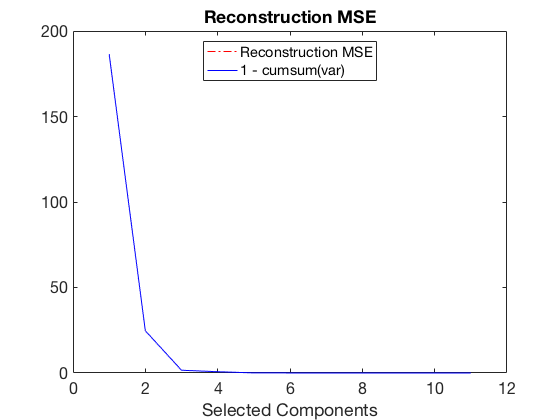
\includegraphics[width=1\linewidth]{./project/wine_rec_MSE.png}
    \end{subfigure}
    \caption{Scaled eigenvalues for the white wine dataset (left) and
    reconstruction MSE with increasing number of components. Clearly 3
    components make a good summarization of the data; they account for more than
    95\% of the variance}
    \label{fig:l5_PC}
  \end{figure}

  This is not necessary a problem: after all, data is now 3.5 times smaller. 
  Furthermore, when using 6 components (half of the original 11), classification
  accuracy is at 69\%. That means that there are still many features in the data
  that are not relevant for the model, and can be pruned out. So it is possible
  to achieve a good compromise between performance and data compression.

  Finally, I would like to point out that I have achieved significant improvements
  when making the net deeper. Using the same configurations as 
  \autoref{tab:l5_transfer_PC}, and [10 5] hidden units in each layer, I already
  achieved 68\% $CCR$ with 3 PC. This improvement happened on all the settings, 
  but only with two layers. With more layers my model performed worse than using only
  one, not even delivering the majority class.

  \begin{table}[h]
    \centering
    \begin{tabular}{@{}lrrrrrrrrrrrr@{}}
      \toprule
      \multirow{2}{*}{\emph{Nhid}}&& \multicolumn{2}{c}{\texttt{logsig}} &&
        \multicolumn{2}{c}{\texttt{tansig}} && \multicolumn{2}{c}{\texttt{purelin}} 
        && \multicolumn{2}{c}{\texttt{softmax}} \\
      && $CCR$ & $T(s)$ && $CCR$ & $T(s)$ && $CCR$ & $T(s)$ && $CCR$ & $T(s)$ \\
      \midrule
       5 && 0.62 & 0.27 && 0.61 & 0.19 && 0.60 & 0.15 && 0.62 & 0.23 \\
      10 && 0.61 & 0.23 && 0.62 & 0.22 && 0.61 & 0.12 && 0.61 & 0.31 \\
      20 && 0.62 & 0.37 && 0.62 & 0.27 && 0.60 & 0.15 && 0.62 & 0.34 \\
      40 && 0.62 & 0.39 && 0.61 & 0.55 && 0.61 & 0.27 && 0.62 & 0.82 \\
      60 && 0.62 & 0.52 && 0.62 & 0.61 && 0.61 & 0.32 && 0.61 & 1.39 \\
      80 && 0.62 & 0.63 && 0.62 & 0.81 && 0.61 & 0.36 && 0.62 & 2.31 \\
    \bottomrule
  \end{tabular}
  \caption{Classification performance on the reduced white wine dataset (3 PC),
    using a \emph{patternnet} with one hidden layer and trained with 
Resilient Backpropagation.}
  \label{tab:l5_transfer_PC}
  \end{table}

  \begin{figure}[htpb]
    \centering
    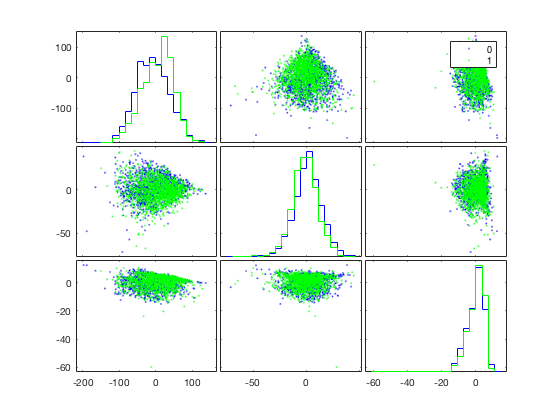
\includegraphics[width=0.7\linewidth]{./project/wine_gplot.png}
    \caption{Gmatrix plot of the reduced white wine dataset. No component
    separates well the classes. Class 0 corresponds to negative class,
  class 1 to the positive 1.}
    \label{fig:l5_wine_gmatrix}
  \end{figure}
    
\end{document}

